\chapter{Interoperability of clouds}

\chapterintro{This chapter introduces the notion of a hybrid cloud and explains its role in IT industry. On top of this deployment model, the concept of InterCloud is presented and elaborated with the emphasis on its application in ensuring scalability of users' services.}

\section{Introduction}
From the perspective of a user of PaaS services it is vital that they are able to deploy seamlessly their applications using libraries, tools and services supported by the cloud provider\cite{MeGr11}. Judging by such factors as the popularity of Heroku -- currently one of the most popular PaaS providers which does not offer more advanced features which would enable management of the infrastructure underpinning the deployment platform, the fact that Microsoft added auto-scaling to its Azure platform as late as in June 2013, it is perfectly possible most PaaS users are satisfied with the current offers of their providers and do need another, more sophisticated functionalities. However, there are more complex applications and systems whose requirements regarding technology stack, availability and scalability are considerably more demanding. For such services there ought to be designed slightly specialized features that would require cooperation among different cloud providers.

\section{Hybrid cloud}
One can imagine scenarios in which customers of cloud services know their applications are vulnerable to sudden variations in demand and their responsiveness must be kept at the same level all the time. In such cases, they want them to scale dynamically according to current load or other predefined or manually specified metrics. What is more, in order to ensure high availability of their services, customers do not want to confine themselves to only one provider -- in the best scenario they want their applications (or their logical parts, such as persistence layer) to be spanned across different providers and be able to cooperate with one another at the same time. This leads to the concept of a \emph{hybrid cloud}\cite{MeGr11} -- the case in which the cloud is a composition of two or more distinct infrastructures which are unique entities, but there are technological means that make it possible to port data and applications among them.

\subsection{Deployment models}
The informal introduction to the concept of a \emph{hybrid cloud} in the previous section requires a strict definition, but it is virtually impossible without defining other deployment models:
\begin{itemize}
  \item Private Cloud -- The provisioned cloud infrastructure is used exclusively by a single organization (that may consist of many business units) and may be owned, managed and operated by the organization or a third party.
  \item Public Cloud -- The provisioned cloud infrastructure is used by general public and may be owned, managed and operated by a business, academic or government organization or some combination of them. It exists on the premises of the cloud provider.
  \item Community Cloud -- The cloud infrastructure is provisioned for exclusive use by a specific community of consumers from organizations that have shared concerns (e.g., mission, security requirements, policy , and compliance considerations). It may be owned, managed , and operated by one or more of the organizations in the community, a third party, or some combination of them, and it may exist on or off premises. 
\end{itemize}
Having defined those models, we can see that \emph{hybrid cloud} can be placed among them and be defined as a model in which the provisioned infrastructure is a composition of two or more other infrastructures - \emph{private},\emph{community} or \emph{public}.

\subsection{Current usage and trends}
\subsubsection*{Cloud -- clients' view}
Before digging into the details of current usage and popularity of the hybrid model, it is worth discussing the general attitude of clients towards cloud computing. As the recent survey \cite{RackspaceSurvey13} shows, the major factor that prevents companies from adopting cloud solutions is their concern over security -- in 2012 as much as 52\% responders considered it as a main concern with the regard to cloud in general. However, the tendency is that more and more enterprises do not find it a major issue as in 2012 the number declined to 46\%.
Complexity related to the managament of cloud components, Vendor lock-in, interoperability and reliability were among the most frequent obsctacles to adoption in 2013 for they constitued 46\%, 35\%, 27\% and 22.3\% of responders' votes respectively. Total results are shown in the figure \ref{ch4:cloud-computing-adoption-obstacles-2013}.
\begin{figure}[!ht]
  \begin{center}
    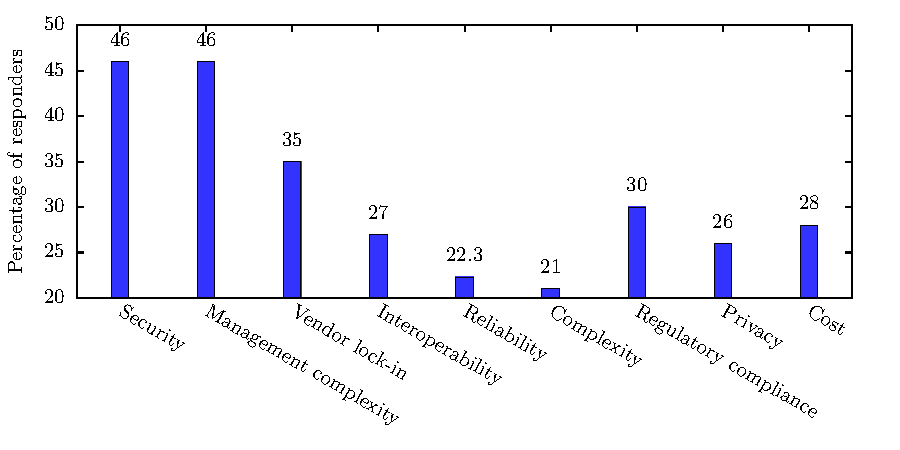
\includegraphics{chapter-4/cloud-computing-adoption-obstacles-2013}
  \end{center}
  \caption{Major obstacles to cloud adoption in 2013 according to \cite{RackspaceSurvey13}}
  \label{ch4:cloud-computing-adoption-obstacles-2013}
\end{figure}

\subsubsection*{View on hybrid cloud}

\section{Federation of clouds -- InterCloud}

\subsection{Usage in industry}

